\documentclass{beamer}
\usetheme[block=fill]{metropolis}%,numbering=none

\usepackage{tikz-cd}
\usepackage{tabu}
\usepackage{listings}
\usepackage{listingsutf8}
\usepackage{epigraph}
\usepackage{graphicx}

\lstset{frame=single, basicstyle=\ttfamily}

\setbeamercolor{section in head/foot}{fg=green}
\definecolor{dark-purple}{RGB}{58,50,135}
\definecolor{darker-blue}{RGB}{6,97,169}
\definecolor{lighter-blue}{RGB}{0,134,179}
\definecolor{teal}{RGB}{131,199,170}

\setbeamercolor{frametitle}{bg=darker-blue}
\setbeamercolor{title separator}{fg=darker-blue}
\setbeamercolor{progress bar}{fg=darker-blue}

\title{A glance at Haskell}
\date{December 2, 2021}
\author{fyusuf-a}
\institute{School 42Paris}



\begin{document}

\maketitle

\section{Learn haskell in 10 minutes}

\begin{frame}{Program 1} %add
	\only<1> {
		\noindent\fbox{%
			\parbox{\textwidth}{%
			\texttt{whoAmI :: \textcolor{red}{Int} -> \textcolor{darker-blue}{Int} -> \textcolor{green}{Int}}

			\texttt{whoAmI \textcolor{red}{x} \textcolor{darker-blue}{y} = \textcolor{green}{x + y}}
			}%
		}
	}
	\only<2-> {
		\noindent\fbox{%
			\parbox{\textwidth}{%
			\texttt{add :: \textcolor{red}{Int} -> \textcolor{darker-blue}{Int} -> \textcolor{green}{Int}}

			\texttt{add \textcolor{red}{x} \textcolor{darker-blue}{y} = \textcolor{green}{x + y}}
			}%
		}
}

\onslide<3->{add 5 3 = }\onslide<4->{5 + 3 = 8}

\onslide<5->{add 10 :: }\onslide<6->{Int -> Int}

\onslide<7->{(add 10) 3 = }\onslide<8->{13}

\end{frame}

\begin{frame}{Program 2 -- recursivity in Haskell} %factorial
	\only<1> {
		\lstinputlisting[language=haskell]{assets/code-examples/program2.hs}
	}
	\only<2-> {
		\lstinputlisting[language=haskell]{assets/code-examples/program2-solution.hs}

		$$factorial n = n! = n\times(n-1)\times\cdots\times1$$
	}
\end{frame}

\begin{frame}{Side note -- precedence}
	factorial 2 - 2 = \onslide<2->{2 * 1 - 2} \onslide<3->{= 0}

	factorial (2 - 2) = \onslide<4->{factorial 0} \onslide<5->{= 1}
\end{frame}

\begin{frame}{Program 3}
	\only<1> {
		\lstinputlisting[language=haskell]{assets/code-examples/program3.hs}
	}
	\only<2-> {
		\lstinputlisting[language=haskell]{assets/code-examples/program3-solution.hs}
	}

	\onslide<3->{orcish "hello" =} \onslide<4->{"hfeflflfof"}
\end{frame}

\begin{frame}{Program 4}
	\lstinputlisting[language=haskell]{assets/code-examples/program4.hs}

	yell (orcish "hello") = \onslide<3->{"hfeflflfof!"}
\end{frame}

\begin{frame}{Program 5}
	\only<1> {
		\lstinputlisting[language=haskell]{assets/code-examples/program5.hs}
	}
	\only<2-> {
		\lstinputlisting[language=haskell]{assets/code-examples/program5-solution.hs}
	}

	\onslide<5->{enthusiastically yell "hello" =} \onslide<6->{"hello!!!"}

	\onslide<7->{yell (orcish "hello") =} \onslide<8->{"hfeflflfof!"}
\end{frame}

\begin{frame}{True Orcish is subtle}
\onslide<1->{very orcish "hello" =} \onslide<2->{"hfffffffeffffffflffffffflfffffffofffffff"}

\onslide<3->{orcish (enthusiastically yell "hello") =} \onslide<4->{"hfeflflfof!f!f!f"}

\end{frame}

\begin{frame}{True Orcish is hardcore}
\onslide<4->{very very orcish "hello" =} \onslide<5->{"hfffffffffffffffffffffffffffffffffffffffffffffffffffffffffffffffffffffffffffffffffffffffffffffffff\newline ffffffffffffffffffffffffffffffffffffffffffffffffffffffffffffffffffffffffffffffffffffffffffffffff\newline ffffffffffffffffffffffffffffffffffffffffffffffffffffffffffffffffffffffffffffffffffffffffffffffff\newline ffffffffffffffffffffffffffffffffffffffffffffffffffffffffffffffffffffffffffffffffffffffffffffffff\newline ffffffffffffffffffffffffffffffffffffffffffffffffffffffffffffffffffffffffffffffffffffffffffffffff\newline ffffffffffffffffffffffffffffffffffffffffffffffffffffffffffffffffffffffffffffffffffffffffffffffff"}

\end{frame}
\begin{frame}{Cross section of an orc}
	
\includegraphics[scale=0.65]{assets/images/incomplete.png}
\end{frame}

\begin{frame}{Sociology of the orcish society}
	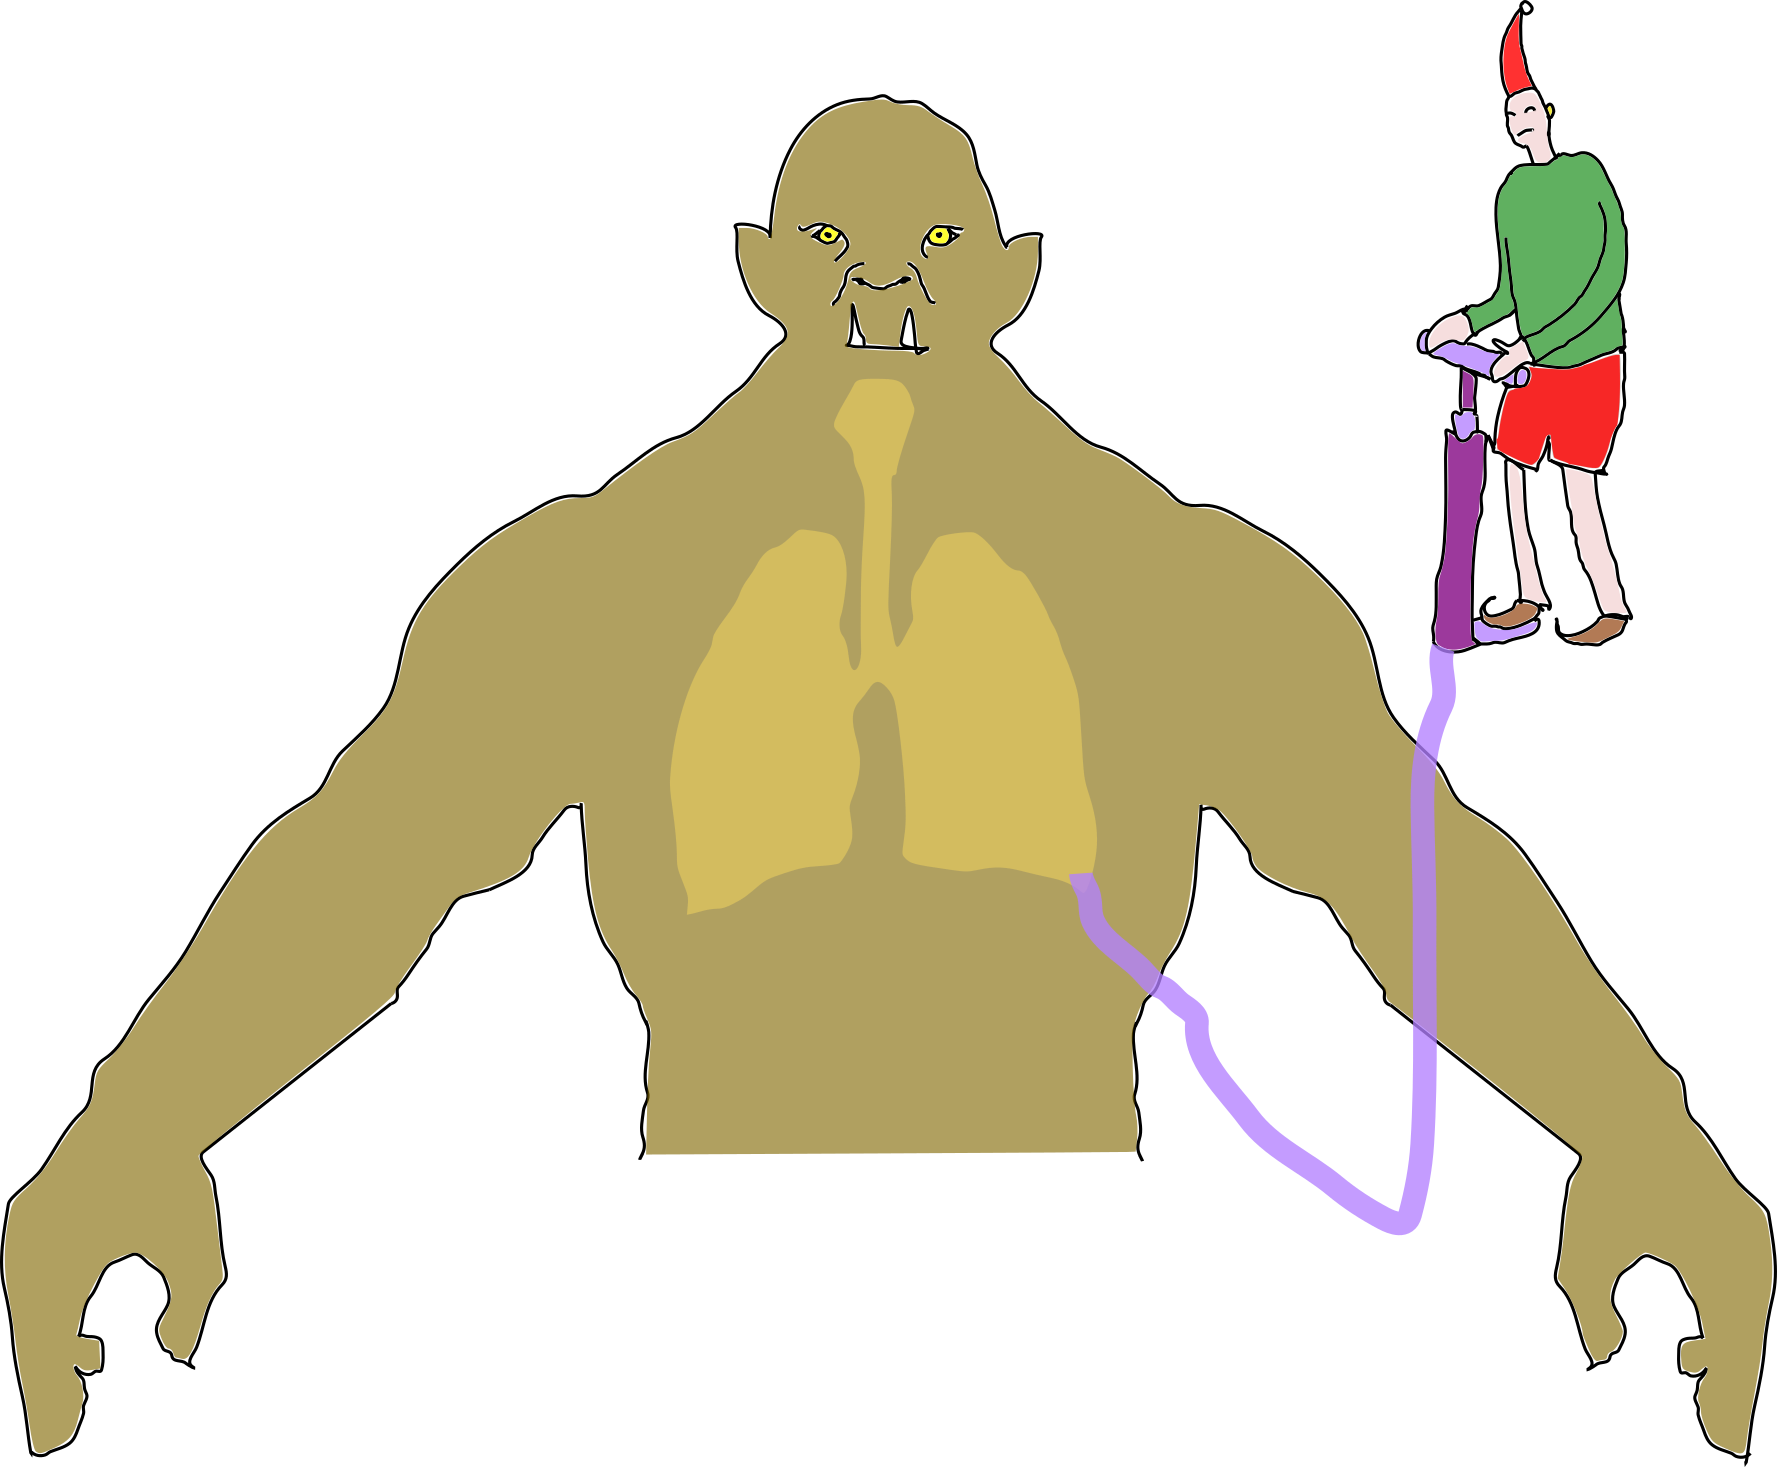
\includegraphics[scale=0.65]{assets/images/complete.png}
\end{frame}
	

\section{Haskell is strongly-typed}

\begin{frame}{Why compile-time checks are important}
	\lstinputlisting[language=Python]{assets/code-examples/hello.py}
\end{frame}

\begin{frame}{Why compile-time checks are important}
	\lstinputlisting[language=Haskell]{assets/code-examples/hello.hs}
\end{frame}

\begin{frame}[fragile]{Why compile-time checks are important}
\begin{verbatim}
hello.hs:8:5: error:
    Variable not in scope: undefined_function :: IO ()
  |
8 |     undefined_function
  |     ^^^^^^^^^^^^^^^^^^
\end{verbatim}
\end{frame}

\begin{frame}{The power of type inference}
	\lstinputlisting[language=Haskell]{assets/code-examples/inference.hs}

	\onslide<2->{
		\lstinputlisting[language=Haskell]{assets/code-examples/inference-ghci.hs}
	}

\end{frame}


\section{Purity in Haskell}

\begin{frame}{A benign C code}
	\lstinputlisting[language=C++]{assets/code-examples/purity.c}
\end{frame}

\begin{frame}{A redflag in Haskell}
	\lstinputlisting[language=haskell]{assets/code-examples/purity.hs}
\end{frame}

\begin{frame}{The Ultimate Question of Life, the Universe and Everything}
	Haskell's answer : ``Separate pure and impure code and minimize impure code.''
\end{frame}

\begin{frame}{But why?}
	Testing becomes easier, and\ldots

	\onslide<2>{one can have lazy evaluation!}
\end{frame}

\section{Haskell is lazy}

\begin{frame}{Yet another riddle}
	\lstinputlisting[language=haskell]{assets/code-examples/take-unanswered.hs}
\end{frame}

\begin{frame}{Yet another riddle}
	\lstinputlisting[language=haskell]{assets/code-examples/take-solution.hs}

	\onslide<2->{take 0 [4, 5, 1] =} \onslide<3->{[]}

	\onslide<4->{take 3 [] =} \onslide<5->{[]}

	\onslide<6->{take 1 [2, 4] =} \onslide<7->{2:take 0 [4] =} \onslide<7->{2:[] = [2]}

\end{frame}


\begin{frame}{Every breath you take}
	\lstinputlisting[language=haskell]{assets/code-examples/take-solution.hs}

	take 2 [1, 4, 5] = \onslide<2->{1:take 1 [4, 5]}

	\onslide<3->{= 1:[4] = [1, 4]}
\end{frame}

\begin{frame}{The list of every natural numbers}
	\lstinputlisting[language=haskell]{assets/code-examples/laziness.hs}

	\onslide<2->{take 1 nat = } \onslide<3->{[0]}

	\onslide<4->{take 5 nat = } \onslide<5->{[0, 1, 2, 3, 4]}
\end{frame}


\begin{frame}{$\infty$ ???}
	\lstinputlisting[language=haskell]{assets/code-examples/laziness.hs}

	\onslide<2->{take 2 nat = } \onslide<3->{take 2 (natConstructor 0)}

	\onslide<4->{= take 2 (0:natConstructor 1)}

	\onslide<5->{= 0:take 1 (natConstructor 1) = } \onslide<6->{0:1:take 0 (natConstructor 2)}

	\onslide<7->{= 0:1:[] =} \onslide<8->{[0, 1]}
\end{frame}

\section{Haskell is concise}

\begin{frame}{Haskell expressivity (1/2)}
	\lstinputlisting[language=haskell]{assets/code-examples/quicksort.hs}
\end{frame}

\begin{frame}[fragile]{Haskell expressivity (2/2)}

\begin{verbatim}
-- Sort all the characters in all strings,
-- across word boundaries!
>>> ("one", "two", "three") & partsOf (each . traversed)
       %~ sort
("eee","hno","orttw")

-- Flip the 2nd bit of each number to a 0
>>> [1, 2, 3, 4] & traversed . bitAt 1 %~ not
[3,0,1,6]
\end{verbatim}
\end{frame}

\section{Real life Haskell}

\begin{frame}{A scraper of Hacker News' API}

	Java : 293 lines and 7547 characters

	\onslide<2->{$\simeq$ 26 characters per line}

	Haskell : 155 lines 5541 characters

	\onslide<2->{$\simeq$ 35 characters per line}

	\vspace{2cm}

	\onslide<3->{
	\texttt{\$ ./benchmark.sh 10}

	\texttt{Mean of fyusuf-a for contest (10 tries): 3.24s}

	\texttt{Mean of ******** for contest (10 tries): 5.00s}
}
\end{frame}

\begin{frame}{Haskell is only for mathematicians ?}
	\begin{itemize}
		\item<2-> Facebook: anti-spam filter and lex-pass, a tool for manipulating a PHP database;
		\item<3-> Google: Ganeti, a tool for managing clusters of virtual servers;
		\item<4-> Microsoft: Bond, their production data serialization framework;
		\item<5-> countless others\ldots
	\end{itemize}
\end{frame}

\begin{frame}{Use cases}

	Haskell is a general-purpose language and has great libraries for almost anything\ldots

	\onslide<2->{\ldots\ but from my meager experience, it seems more difficult to do numeric calculations and mobile development.}
	
\end{frame}

\begin{frame}{Thanks}

	\begin{itemize}
		\item Chris Penner, for the examples of expressivity using lenses;
		\item FrungyKing, for his Youtube video and his jokes on Swedish;
		\item Junior 42Paris for the organization.
	\end{itemize}

\end{frame}

\end{document}
